\documentclass[11pt,a4paper]{article}
\usepackage[T1]{fontenc}
\usepackage{lmodern}
\usepackage{amsmath,amssymb,amsthm}
\usepackage[margin=25mm]{geometry}
\usepackage{booktabs}
\usepackage{graphicx}
\usepackage{microtype}
\usepackage[hidelinks]{hyperref}
\usepackage{xurl}

\newtheorem{theorem}{Theorem}[section]
\newtheorem{lemma}[theorem]{Lemma}
\newtheorem{proposition}[theorem]{Proposition}
\newtheorem{corollary}[theorem]{Corollary}
\theoremstyle{definition}
\newtheorem{definition}[theorem]{Definition}
\newtheorem{remark}[theorem]{Remark}
\numberwithin{equation}{section}

\newcommand{\C}{\mathbb C}
\newcommand{\R}{\mathbb R}
\newcommand{\tr}{\operatorname{tr}}

\title{How badly can column-pivoted QR choose rows of an orthonormal basis?\\[2pt]
\large The sharp stretched-exponential worst case}
\author{Anonymous}
\date{16 November 2026\\[2pt]\small Version 0.1.0-candidate, DOI \href{https://doi.org/10.5281/zenodo.24278831}{10.5281/zenodo.24278831}}

\begin{document}
\maketitle

\begin{abstract}
Many numerical methods must pick $k$ rows of an $N\times k$ matrix $Q$ with orthonormal columns so that the
selected $k\times k$ block is well conditioned. This is the interpolation-point step of the discrete empirical
interpolation method (DEIM), and it also appears in column-subset selection. The rule used
in practice is classical column-pivoted QR (QRCP) applied to $Q^*$. Its quality is measured by
$\gamma=\|Q(I,:)^{-1}\|_2$, the factor by which interpolation can exceed the best possible error. A selection with
$\gamma\le\sqrt{k(N-k+1)}$ always exists. The classical guarantee for QRCP grows like $2^k$, however. Chen, Liu, He
and Dong (2026) showed that QRCP can do worse than every polynomial multiple of the existence scale, even when all
rows have comparable energy, and their construction already gives growth of order $\exp(c\sqrt k)$.

This paper determines the worst case on the logarithmic scale. Let the coherence $\mu(Q)$ be the largest row energy
divided by the average. If $\mu(Q)\le H$, then every legal QRCP selection satisfies
$\gamma\le\sqrt{e(N-k+1)}\,\exp(C(H)\sqrt k)$. Here $C(H)$ is an explicit constant: it equals $2$ when all rows
have equal energy and grows like $\sqrt{\log H}$. Matching examples show that $C(H)$ cannot be lowered, including at
exactly equal row energies (there under a specified tie-breaking rule). Coherence never exceeds $N/k$, so the bound needs no assumption at all if $C(N/k)$ is
used. In particular, for $N\ge2k$ QRCP is never worse than the existence scale by more than
$\exp(O(\sqrt{k\log(N/k)}))$. This order is attained when $k^{2+\varepsilon}\le N\le e^{o(k)}$, and the exact leading
constant is attained when $\log N/\log k\to\infty$ with $\log N=o(k)$. A by-product is an a posteriori bound in terms of the
observed pivot sizes, with an optimal leading coefficient. All results concern exact arithmetic and worst cases.
Whether growth of order $\exp(c\sqrt k)$ can occur when $N$ is a fixed multiple of $k$ remains open.
\end{abstract}

\noindent\textbf{Keywords:} column-pivoted QR; discrete empirical interpolation; coherence; Kahan matrix;
triangular inverse; worst-case analysis.

\noindent\textbf{MSC 2020:} 65F25, 65F35, 15A12, 15A23.

%=====================================================================
\section{Introduction}\label{sec:intro}

This section explains the problem, what was known, what is new and how the paper is organised.

\subsection{The problem}
Suppose the columns of $Q\in\C^{N\times k}$ form an orthonormal basis of a $k$-dimensional space of vectors of
length $N$, for example $k$ dominant modes of a simulation sampled at $N$ grid points. Many algorithms need $k$
of the $N$ coordinates (rows) such that the selected square block $Q(I,:)$ is well conditioned. In DEIM and its
QR-based variant Q-DEIM, a vector $f$ is approximated from its values at the selected coordinates only, by the
interpolant $\mathcal D f=Q\,Q(I,:)^{-1}f(I)$. The error then satisfies
\begin{equation}\label{eq:intro-deim}
  \|f-\mathcal D f\|_2\le \gamma(Q,I)\,\|f-QQ^*f\|_2,\qquad \gamma(Q,I)=\|Q(I,:)^{-1}\|_2,
\end{equation}
and $\gamma$ is exactly the norm of $I-\mathcal D$ (Section~\ref{sec:interp}). So $\gamma$ is the factor by which
interpolation can lose against the best approximation from the same space. The same quantity governs the
Golub--Klema--Stewart column-subset method and the stability of greedy point selection [DG16, A26, D26].

The rule most used in practice is classical \emph{column-pivoted QR} (QRCP, also called Businger--Golub pivoting)
applied to $Q^*$. At each step it projects the remaining columns of $Q^*$ away from those already chosen and takes
the one with the largest residual norm. In the language of rows of $Q$: it repeatedly picks the coordinate that is
least explained by the coordinates already chosen. Equivalently, it is greedy diagonal-pivoted Cholesky
factorisation of the orthogonal projector $QQ^*$ [DG16, proof of Theorem~2.1]. It is cheap and is available in every dense linear-algebra
library. The question is how large $\gamma$ can be for the rows that this greedy rule picks.

\subsection{What was known}
\begin{itemize}
\item \emph{Existence.} Some choice of rows always has $\gamma\le\sqrt{k(N-k+1)}$; this is the benchmark
  (``existence scale'') used in the problem statement of Amsel et al.\ [A26, Section 4.1.2], which records the
  existence result and an efficient algorithm achieving it.
\item \emph{Classical upper bound for QRCP.} Drmač and Gugercin [DG16, Theorem~2.1] proved
  $\gamma\le\sqrt{N-k+1}\,\sqrt{4^k+6k-1}/3$, which grows like $2^k$. Their proof uses the greedy inequalities one
  matrix entry at a time. Kahan's classical triangular matrix [K66] shows that inequalities of this type alone allow
  exponential growth, but Kahan's matrix does not have orthonormal rows.
\item \emph{The open question.} Damle and Kressner asked whether QRCP satisfies the existence bound, or a similar
  one, when the input has orthonormal rows [A26, Problem~4.3].
\item \emph{Engler's analysis.} Engler [E97] proved the pivot lower bound used in Lemma~\ref{lem:suffix} below,
  showed that QRCP on orthonormal rows achieves at least the average determinant, and gave examples with coherence
  tending to one, completed with Hadamard matrices, whose selected blocks have condition number growing like
  $\sqrt{k\log k}$.
\item \emph{The negative answer.} Chen, Liu, He and Dong [CLHD26, Theorem~2 and Appendix~B] answered Problem~4.3
  negatively. For every coherence cap $H_*>1$ they built orthonormal inputs on which $\gamma$ exceeds every
  polynomial multiple of $\sqrt{k(N-k+1)}$. Their Lemma~24 in fact gives growth $\exp(c\sqrt k)$ up to polynomial
  factors, for every $c<\tfrac12\sqrt{\log H_*}$ (Remark~\ref{rem:chen}). A finite exact example with $k=3$, $N=8$
  is recorded by Count ex Machina [S26, Appendix~A.5].
\item \emph{A different rule.} Damle [D26, Theorem~3.1 and Corollary~3.2] showed that the Bischof--Stewart pivoting
  rule achieves $\gamma\le\sqrt{1+k(N-k)}$ on orthonormal rows (the bound on $\gamma$ itself is due to Osinsky,
  as [D26] records). The update to [A26] (version~3, Problem~4.3)
  records both the negative answer for QRCP and this positive answer for the modified rule.
\end{itemize}
Related work on scaled triangular inverses [DV08] and on the approximation error of pivoted QR under
singular-value decay [G26] concerns different quantities.
So before this paper the worst case of classical QRCP on orthonormal rows was known to lie between
$\exp(c\sqrt k)$ and $2^k$, with no upper bound below exponential.

\subsection{What is new}
Write $\mu(Q)=(N/k)\max_j\|Q(j,:)\|_2^2$ for the coherence: the largest row energy relative to the average $k/N$.
Thus $1\le\mu(Q)\le N/k$, and $\mu(Q)=1$ means that every row carries the same energy.
\begin{enumerate}
\item \emph{A stretched-exponential upper bound} (Theorem~\ref{thm:main}). If $\mu(Q)\le H$, every legal QRCP
  selection, with any tie-breaking, satisfies
  \[
    \gamma(Q,I)\le\sqrt{e(N-k+1)}\,\exp\bigl(C(H)\sqrt k\bigr),
  \]
  with the explicit constant $C(H)$ of \eqref{eq:CH} (Table~\ref{tab:CH}). To our knowledge this is the first bound for
  QRCP on orthonormal rows that is below exponential in $k$.
\item \emph{The constant is sharp} (Theorem~\ref{thm:main}). For every fixed $H\ge1$ the worst case $G_k(H)$ of
  $\gamma/\sqrt{N-k+1}$ (defined in \eqref{eq:Gk}) satisfies $\log G_k(H)=(C(H)+o(1))\sqrt k$. The matching examples are real, have fewer than $3k^3$ rows, and have unique
  pivots when $H>1$. At $H=1$ (exactly equal row energies) a matching family exists under the smallest-label
  tie rule. For comparison, the construction of [CLHD26] reaches coefficients below $\tfrac12\sqrt{\log H}$, which
  tends to $0$ as $H\downarrow1$, whereas $C(H)\ge2$.
\item \emph{No assumption needed} (Corollary~\ref{cor:free}). Since $\mu(Q)\le N/k$, every orthonormal input
  satisfies $\gamma\le\sqrt{e(N-k+1)}\exp(C(N/k)\sqrt k)$. At a fixed aspect ratio $N\le\alpha k$ the growth is at
  most $\exp(C(\alpha)\sqrt k)$; for instance $C(2)\approx2.248$.
\item \emph{The law in $N$ and $k$} (Theorem~\ref{thm:Nk} and Corollary~\ref{cor:law}). Without any coherence
  assumption, the worst case is $\exp(\Theta(\sqrt{k\log(N/k)}))$ once $N\ge k^{2+\varepsilon}$ (and $\log N=o(k)$),
  and it is $\exp((1+o(1))\sqrt{k\log N})$ when $\log N/\log k\to\infty$.
\item \emph{An a posteriori bound} (Theorem~\ref{thm:range}). In terms of the observed pivot range
  $L=\log(d_1^2/d_k^2)$, where $d_1\ge\dots\ge d_k$ are the diagonal entries of the triangular factor, one has $\gamma\le(\sqrt e/d_k)\exp(\sqrt{(k-1)L})$, and the coefficient one is optimal
  (Proposition~\ref{prop:range-sharp}).
\end{enumerate}
Table~\ref{tab:DG} shows what the new bound means at practical sizes. It is smaller than the Drmač--Gugercin
factor from $k=13$ (for $H=1$) or $k=15$ (for $H=2$) onwards. At $k=100$ it allows about $10^{9}$ to $10^{10}$ where
the classical bound allowed $10^{30}$.

\begin{table}[t]
\centering
\caption{The sharp constant $C(H)$ of \eqref{eq:CH}. As $H\to\infty$, $C(H)^2/\log H\to1$, slowly.}\label{tab:CH}
\begin{tabular}{lcccccc}
\toprule
$H$ & 1 & 1.5 & 2 & 4 & 10 & 100\\
$\rho(H)$ & 1 & 2.1888 & 2.6783 & 3.6926 & 4.8897 & 7.6384\\
$C(H)$ & 2 & 2.1554 & 2.2476 & 2.4420 & 2.6635 & 3.1256\\
\bottomrule
\end{tabular}
\end{table}

\begin{table}[t]
\centering
\caption{Base-10 logarithm of the factor multiplying $\sqrt{N-k+1}$ in the classical bound of [DG16] and in the new
bound $\sqrt e\exp(C(H)\sqrt k)$. The new bound is smaller from $k=13$, $15$, $20$ and $25$ onwards for
$H=1$, $2$, $10$ and $100$ respectively.}\label{tab:DG}
\begin{tabular}{rcccc}
\toprule
$k$ & [DG16] & new, $H=1$ & new, $H=2$ & new, $H=10$\\
\midrule
10 & 2.53 & 2.96 & 3.30 & 3.88\\
20 & 5.54 & 4.10 & 4.58 & 5.39\\
50 & 14.57 & 6.36 & 7.12 & 8.40\\
100 & 29.63 & 8.90 & 9.98 & 11.78\\
200 & 59.73 & 12.50 & 14.02 & 16.58\\
\bottomrule
\end{tabular}
\end{table}

\paragraph{The idea in one paragraph.}
Greedy pivoting gives more information than the entrywise inequalities used before: every selected column has
bounded energy in \emph{every} trailing block of coordinates, simultaneously (Lemma~\ref{lem:suffix}). A diagonal
change of scale, chosen to grow quickly while the pivots are large and slowly once they approach the floor imposed
by orthonormality, turns these constraints into a bound on the Frobenius norm of a triangular matrix with unit
diagonal; a determinant argument then bounds its inverse (Sections~\ref{sec:info}--\ref{sec:upper}). The matching
examples use a generalised Kahan matrix whose diagonal follows the same two-part profile (Figure~\ref{fig:main}),
completed to an orthonormal matrix by columns too small to be picked (Sections~\ref{sec:lower}--\ref{sec:endpoint}).

\paragraph{What the paper does not claim.}
The results concern exact arithmetic. They describe worst cases, not typical inputs, on which QRCP usually performs
well. The constant $C(H)$ is sharp on the logarithmic scale; the upper and lower bounds still differ by a factor
that is polynomial in $k$ at fixed $H$, and the limits are approached slowly (Section~\ref{sec:scope}). The
worst-case examples have $N$ of order $k^3$; what happens at $N=O(k)$ is open.

\paragraph{Roadmap.}
Section~\ref{sec:results} sets out definitions and states the main results. Section~\ref{sec:info} records what
greedy pivoting guarantees, and Section~\ref{sec:upper} proves the upper bound. Sections~\ref{sec:lower}
and~\ref{sec:endpoint} build the matching examples, first for $H>1$ and then at $H=1$; Appendix~\ref{app:A} makes
the $H=1$ construction quantitative. Section~\ref{sec:range} proves the a posteriori bound and the law in $N$ and
$k$. Section~\ref{sec:interp} explains the consequence for interpolation and gives practical guidance.
Section~\ref{sec:scope} reports the computational checks and lists open problems.

%=====================================================================
\section{Setting and main results}\label{sec:results}

This section fixes notation and states the theorems; proofs follow in later sections.

All logarithms are natural. $\|\cdot\|$ is the Euclidean (spectral) norm and $\|\cdot\|_F$ the Frobenius norm.
Throughout, $N\ge k$ and $Q\in\C^{N\times k}$ with $Q^*Q=I_k$; equivalently $W=Q^*$ has orthonormal rows.

\begin{definition}[QRCP and legal selections]
\emph{Exact QRCP} on $W=Q^*$ runs for $k$ steps. At each step it projects every unselected column of $W$ onto the
orthogonal complement of the span of the columns already selected, and selects a column whose projection
(residual) has the largest norm. When several columns tie, any of them may be taken; each resulting ordered index
tuple $I=(i_1,\dots,i_k)$ is a \emph{legal selection}. Since $W$ has rank $k$, the selected columns are independent,
and $\gamma(Q,I)=\|Q(I,:)^{-1}\|$ is finite.
\end{definition}

\begin{definition}[coherence and the constant $C(H)$]
The coherence is
\begin{equation}\label{eq:coh}
  \mu(Q)=\frac Nk\max_{1\le j\le N}\|Q(j,:)\|_2^2\in[1,N/k].
\end{equation}
For $H\ge1$ let $\rho=\rho(H)\ge1$ be the solution of
\begin{equation}\label{eq:CH}
  \rho-\log\rho=1+\log H,\qquad\text{and put}\qquad C(H)=\sqrt{\rho}+\frac1{\sqrt{\rho}}.
\end{equation}
Then $\rho(1)=1$ and $C(1)=2$; $C$ is continuous and increasing; and $C(H)^2=\rho+2+1/\rho$ with
$\rho=\log H+\log\log H+O(1)$ as $H\to\infty$. In closed form $\rho=-W_{-1}(-1/(eH))$, with $W_{-1}$ the lower branch
of the Lambert function.
\end{definition}

For $k\ge2$ and $H\ge1$ the worst case, normalised by the factor $\sqrt{N-k+1}$ of the classical bound, is
\begin{equation}\label{eq:Gk}
 G_k(H)=\sup\Bigl\{\frac{\gamma(Q,I)}{\sqrt{N-k+1}}:\ N\ge k,\ Q\in\C^{N\times k},\ Q^*Q=I_k,\ \mu(Q)\le H,\
 I\text{ a legal selection}\Bigr\}.
\end{equation}
The number of rows $N$ is free in this supremum.

\begin{theorem}[sharp growth at bounded coherence]\label{thm:main}
For every $H\ge1$, every $k\ge2$, every $Q$ with $Q^*Q=I_k$ and $\mu(Q)\le H$, and every legal selection $I$,
\begin{equation}\label{eq:upper}
 \gamma(Q,I)\le\sqrt{e(N-k+1)}\,\exp\bigl(C(H)\sqrt k\bigr).
\end{equation}
For every fixed $H\ge1$,
\begin{equation}\label{eq:limit}
  \lim_{k\to\infty}\frac{\log G_k(H)}{\sqrt k}=C(H).
\end{equation}
For $H>1$ the lower bound is realised by real matrices with $N<3k^3$ and a unique pivot at every step
(Section~\ref{sec:lower}). At $H=1$ it is realised by real matrices with $N=O(k^3\log k)$ under the
smallest-label tie rule (Section~\ref{sec:endpoint} and Appendix~\ref{app:A}).
\end{theorem}

\begin{remark}[what ``sharp'' means here]\label{rem:sharp}
The upper bound \eqref{eq:upper} has an $O(1)$ error in the exponent. For each fixed $\bar H<H$ the examples give
$\log(\gamma/\sqrt{N-k+1})\ge C(\bar H)\sqrt k-O(\log k)$. Thus \eqref{eq:limit} determines the leading term of the
exponent, not a multiplicative constant: at fixed $H$ the two bounds may still differ by a factor polynomial in $k$.
The limit is also approached slowly; see Section~\ref{sec:scope} and Figure~\ref{fig:main}(B). The same limit holds if
$\sqrt{N-k+1}$ in \eqref{eq:Gk} is replaced by $\sqrt N$ or by the existence scale $\sqrt{k(N-k+1)}$, because
$1\le N/(N-k+1)\le k$ and the factor $\sqrt k$ changes the logarithm by $O(\log k)$.
\end{remark}

\begin{remark}[comparison with the construction of Chen et al.]\label{rem:chen}
In [CLHD26, Appendix~B] the selected block is a chain with diagonal $d_t=\epsilon^{t-1}/k$, $\epsilon=e^{-\eta/k}$,
off-diagonal couplings of relative size $\beta s$ with $\beta=\tfrac12$ and $s=(1-\epsilon^2)^{1/2}$, and coherence at
most $e^{2\eta}+o(1)<H_*$ (their Lemma~23). Their Lemma~24 gives $\gamma^2\ge Z/r$ with
$Z\ge\gamma_0^2s^2(1+\beta s)^{2(m-2)}$, and Lemma~25 gives $r(N-k+1)\le3k$. Since $s\sim\sqrt{2\eta/k}$, this yields
$\log\bigl(\gamma/\sqrt{k(N-k+1)}\bigr)\ge\sqrt{\eta/2}\,\sqrt k-O(\log k)$, so every coefficient
$c<\tfrac12\sqrt{\log H_*}$ is reached. This is the stretched-exponential order, with a coefficient that tends to
zero as $H_*\downarrow1$ (for example $0.42$ against $C(2)=2.25$). Their diagonal profile is geometric with total
logarithmic drop $2\eta<\log H_*$ and couplings of half strength. A steeper first branch, full-strength couplings,
and a second branch that follows the floor imposed by orthonormality (profile \eqref{eq:profile}) together raise
the coefficient to $C(H)$.
\end{remark}

Because the coherence of any orthonormal $Q$ is at most $N/k$, Theorem~\ref{thm:main} needs no hypothesis at all.

\begin{corollary}[no coherence assumption]\label{cor:free}
For every $Q\in\C^{N\times k}$ with $Q^*Q=I_k$, $k\ge2$, and every legal selection,
\begin{equation}\label{eq:free}
  \gamma(Q,I)\le\sqrt{e(N-k+1)}\,\exp\Bigl(\min\bigl\{C(N/k)\sqrt k,\ \sqrt{(k-1)\log(N-k+1)}\bigr\}\Bigr).
\end{equation}
In particular, if $N\le\alpha k$ then $\gamma\le\sqrt{e(N-k+1)}\exp(C(\alpha)\sqrt k)$, and since
$C(H)^2\le\log H+\log(1+\log H)+5$, QRCP is never worse than the existence scale by more than
$\exp(\sqrt{k\log(N/k)}(1+o(1)))$ as $N/k\to\infty$.
\end{corollary}

The next theorem shows that this order is attained when $N$ is at least a little larger than $k^2$.

\begin{theorem}[the law in $N$ and $k$]\label{thm:Nk}
For $k\ge2$ and $N\ge k$ let $\Gamma_k(N)$ be the supremum of $\gamma(Q,I)/\sqrt{N-k+1}$ over all $Q\in\C^{N\times k}$
with $Q^*Q=I_k$ (exactly $N$ rows, no coherence assumption) and all legal selections. Then:
\begin{enumerate}
\item[(a)] $\log\Gamma_k(N)\le\tfrac12+\min\{C(N/k)\sqrt k,\ \sqrt{(k-1)\log(N-k+1)}\}$;
\item[(b)] if $k\ge3$ and $L=\log\bigl(N/(66k^2)\bigr)$ satisfies $1\le L\le(k-1)/2$, then
  \begin{equation}\label{eq:Nk-lower}
   \log\Gamma_k(N)\ge\sqrt{kL}-L-\log k-3,
  \end{equation}
  realised by a real generalised Kahan block with unique pivots.
\end{enumerate}
\end{theorem}

\begin{corollary}\label{cor:law}
Let $k\to\infty$ and $N=N_k$.
\begin{enumerate}
\item[(i)] If $\log N/\log k\to\infty$ and $\log N=o(k)$, then $\log\Gamma_k(N)=(1+o(1))\sqrt{k\log N}$.
\item[(ii)] If $N=\lfloor k^\alpha\rfloor$ with fixed $\alpha>2$, then
 \[
  \sqrt{\alpha-2}\le\liminf\frac{\log\Gamma_k(N)}{\sqrt{k\log k}}\le\limsup\frac{\log\Gamma_k(N)}{\sqrt{k\log k}}
  \le\sqrt{\alpha-1}.
 \]
\end{enumerate}
\end{corollary}

\begin{figure}[t]
\centering
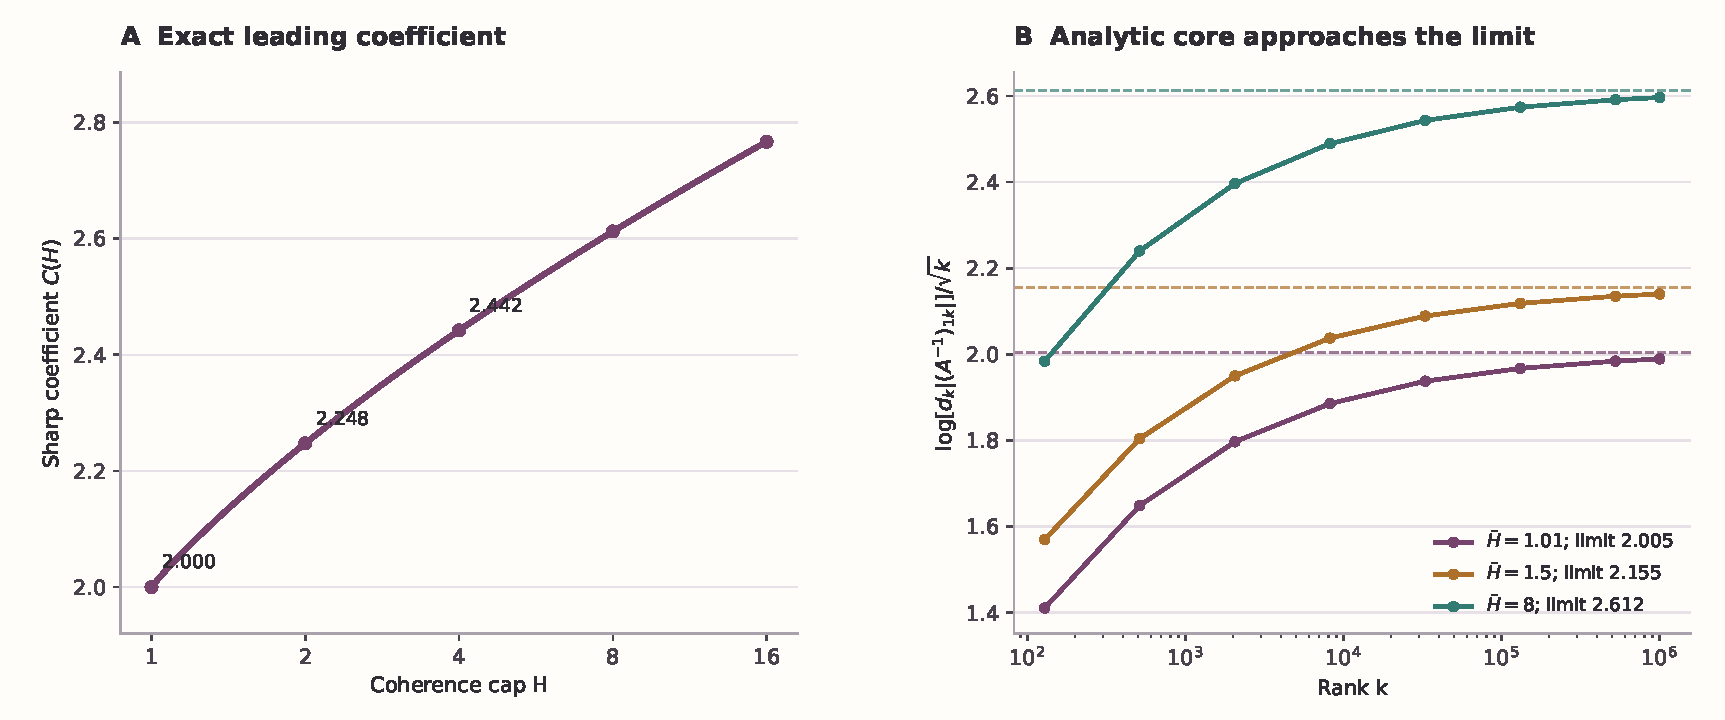
\includegraphics[width=\textwidth]{figures/sharp-growth.pdf}
\caption{(A) The sharp coefficient $C(H)$ of Theorem~\ref{thm:main}. (B) Normalised logarithm of the selected inverse
entry for the triangular core of Section~\ref{sec:lower} at profile parameter $\bar H$, computed in extended (or, on some
platforms, double) precision and checked against 80-digit evaluations, for $k$ up to $10^6$; dashed lines are the limits $C(\bar H)$. Convergence is slow: at
$k=10^6$ the core reaches $2.140$ against the limit $2.155$ for $\bar H=1.5$. Only the triangular cores are evaluated
at large $k$; completed matrices were built and factorised for $k\le128$ (Section~\ref{sec:scope}).}
\label{fig:main}
\end{figure}

%=====================================================================
\section{What greedy pivoting guarantees}\label{sec:info}

This section extracts from the pivot rule all the inequalities used later. The key point is
Lemma~\ref{lem:weighted}: it uses the constraints on every trailing block of every column at once, which is what
the earlier entrywise analyses did not do.

After a unitary change of coordinates on the left and a permutation of columns, write
\[
 Q^*\Pi=U\,[R\ \ Z],
\]
where $R$ is the $k\times k$ upper-triangular block of the selected columns, in the order selected. Its diagonal can
be taken positive; put $d_i=R_{ii}>0$ and $D=\operatorname{diag}(d_i)$. Then $\gamma(Q,I)=\|R^{-1}\|$.

\begin{lemma}[trailing energies and pivot floors]\label{lem:suffix}
The selected block satisfies
\begin{equation}\label{eq:suffix}
 d_1\ge d_2\ge\dots\ge d_k>0,\qquad \sum_{\ell=i}^{j}|R_{\ell j}|^2\le d_i^2\quad(1\le i\le j\le k),
\end{equation}
and
\begin{equation}\label{eq:floor}
 d_i^2\ge\frac{k-i+1}{N-i+1},\qquad d_1^2=\frac{k\,\mu(Q)}{N}.
\end{equation}
\end{lemma}

\begin{proof}
At step $i$ the chosen pivot has residual norm $d_i$. Every selected column $j\ge i$ was available at that step, and
its residual norm then was $(\sum_{\ell=i}^j|R_{\ell j}|^2)^{1/2}$; it cannot exceed the pivot's. This holds for
every tie-breaking. Projecting onto a smaller space cannot increase a norm, which gives monotonicity of the $d_i$.

The rows of $[R\ Z]$ are orthonormal, so its last $k-i+1$ rows have total squared Frobenius norm $k-i+1$. Their first
$i-1$ columns vanish, and each of the other $N-i+1$ columns has squared norm at most $d_i^2$ in these rows, because
$d_i$ is the largest residual at step $i$. This proves the first part of \eqref{eq:floor}; the same argument appears
in Engler [E97, proof of Theorem~2]. The first pivot is a longest column of $Q^*$, that is, a row of $Q$ of largest
energy, which gives the formula for $d_1$.
\end{proof}

Set $t_i=\log(d_1^2/d_i^2)$, the logarithmic drop of the $i$-th pivot. If $\mu(Q)\le H$, Lemma~\ref{lem:suffix}
gives the \emph{barrier}
\begin{equation}\label{eq:barrier}
 0=t_1\le t_2\le\dots\le t_k,\qquad t_i\le\log\frac{Hk}{k-i+1},
\end{equation}
since $d_1^2/d_i^2\le (kH/N)(N-i+1)/(k-i+1)\le Hk/(k-i+1)$.

\begin{lemma}[weighted trailing-energy estimate]\label{lem:weighted}
Let $R$ satisfy \eqref{eq:suffix}, and let $w:[0,t_k]\to\R$ be nondecreasing. Put
\[
 V=\operatorname{diag}\bigl(e^{w(t_i)}\bigr),\qquad B=VD^{-1}RV^{-1}.
\]
Then $B$ is upper triangular with unit diagonal, and for $j\ge2$
\begin{equation}\label{eq:weighted}
 \sum_{i<j}|B_{ij}|^2\le\int_0^{t_j}\exp\bigl\{-2[w(t_j)-w(t)]\bigr\}\,dt.
\end{equation}
If moreover $w$ is continuously differentiable and concave with $w'>0$, then
\begin{equation}\label{eq:weighted-concave}
 \sum_{i<j}|B_{ij}|^2\le\frac1{2w'(t_j)}.
\end{equation}
\end{lemma}

\begin{proof}
Fix $j$. Write $a_i=d_i^2$, $x_i=|R_{ij}|^2$ for $i<j$, and $S_i=\sum_{\ell=i}^{j-1}x_\ell$. By \eqref{eq:suffix},
$S_i\le a_i-a_j$. The weights $W_i=a_i^{-1}e^{2w(t_i)}=d_1^{-2}e^{t_i+2w(t_i)}$ are nondecreasing in $i$. Summation
by parts therefore gives
\[
\begin{aligned}
 \sum_{i<j}W_ix_i&=W_1S_1+\sum_{i=2}^{j-1}(W_i-W_{i-1})S_i
 \le\sum_{i<j}W_i(a_i-a_{i+1})\\
 &=\sum_{i<j}e^{2w(t_i)}\bigl(1-e^{-(t_{i+1}-t_i)}\bigr)
 \le\int_0^{t_j}e^{2w(t)}\,dt,
\end{aligned}
\]
using $S_i\le a_i-a_j$, a telescoping rearrangement, $1-e^{-x}\le x$, and monotonicity of $w$ on each interval
$[t_i,t_{i+1}]$. Since $|B_{ij}|^2=e^{2w(t_i)-2w(t_j)}x_i/a_i=e^{-2w(t_j)}W_ix_i$, multiplying by $e^{-2w(t_j)}$ proves
\eqref{eq:weighted}. If $w$ is concave, $w(t_j)-w(t)\ge w'(t_j)(t_j-t)$ for $t\le t_j$; integrating the resulting
exponential gives \eqref{eq:weighted-concave}.
\end{proof}

The last ingredient is a classical determinant estimate; we include its two-line proof and claim no novelty for it.

\begin{lemma}[determinant and Frobenius norm]\label{lem:det}
Let $B$ be a $k\times k$ matrix with $|\det B|=1$, $k\ge2$, and $\|B\|_F^2=k+E$. Then
\begin{equation}\label{eq:det}
 \|B^{-1}\|\le\Bigl(\frac{k+E}{k-1}\Bigr)^{(k-1)/2}\le\exp\Bigl(\frac{E+1}2\Bigr).
\end{equation}
\end{lemma}

\begin{proof}
Let $\sigma_1\ge\dots\ge\sigma_k$ be the singular values. Since their product is one, the arithmetic--geometric mean
inequality gives $\sigma_k^{-2}=\prod_{i<k}\sigma_i^2\le\bigl(\sum_{i<k}\sigma_i^2/(k-1)\bigr)^{k-1}\le((k+E)/(k-1))^{k-1}$.
Use $1+x\le e^x$ with $x=(E+1)/(k-1)$ and take square roots.
\end{proof}

%=====================================================================
\section{Proof of the upper bound}\label{sec:upper}

This section proves \eqref{eq:upper} by choosing the weight $w$ in Lemma~\ref{lem:weighted}. There is a trade-off:
a fast-growing $w$ makes the off-diagonal part of $B$ small, but the similarity $V$ then has a large condition
number. The barrier \eqref{eq:barrier} says that late pivots are already close to the floor, so the weight can
afford to grow more slowly there.

Fix $b>0$ and $\tau\ge0$ and let
\begin{equation}\label{eq:w}
 w(t)=\begin{cases} bt,&0\le t\le\tau,\\ b\tau+2b\bigl(1-e^{-(t-\tau)/2}\bigr),&t\ge\tau.\end{cases}
\end{equation}
This function is increasing, continuously differentiable and concave, its range is at most $b(\tau+2)$, and
$1/w'(t)=b^{-1}\max\{1,e^{(t-\tau)/2}\}$. By \eqref{eq:barrier} and \eqref{eq:weighted-concave}, with $s=k-j+1$,
\begin{equation}\label{eq:E}
 E:=\|B\|_F^2-k\le\frac1{2b}\sum_{s=1}^k\max\Bigl\{1,\sqrt{\frac{Hke^{-\tau}}s}\Bigr\}\le\frac{k(1+He^{-\tau})}{2b}.
\end{equation}
For the last step put $q=Hke^{-\tau}$: the decreasing function $f_q(x)=(\sqrt{q/x}-1)_+$ has
$\int_0^\infty f_q=q$, so $\sum_{s=1}^kf_q(s)\le q$. No asymptotic approximation is involved.

Since $B$ is unit upper triangular, $\det B=1$. From $R^{-1}=V^{-1}B^{-1}VD^{-1}$, $\|V\|\|V^{-1}\|\le e^{b(\tau+2)}$
and Lemma~\ref{lem:det},
\begin{equation}\label{eq:upper-b}
 \|R^{-1}\|\le\frac{\sqrt e}{d_k}\exp\Bigl\{b(\tau+2)+\frac{k(1+He^{-\tau})}{4b}\Bigr\}.
\end{equation}
Minimising over $b>0$ gives
\begin{equation}\label{eq:upper-tau}
 \|R^{-1}\|\le\frac{\sqrt e}{d_k}\exp\Bigl\{\sqrt{k(\tau+2)(1+He^{-\tau})}\Bigr\}.
\end{equation}
The derivative of $(\tau+2)(1+He^{-\tau})$ is $1-H(\tau+1)e^{-\tau}$. For $H>1$ the unique minimum on $[0,\infty)$ is
at $\tau=\rho(H)-1$; for $H=1$ it is at $\tau=0$. There $He^{-\tau}=1/\rho$, and the square root in
\eqref{eq:upper-tau} equals $\sqrt{k(\rho+1)(1+1/\rho)}=C(H)\sqrt k$. Finally $d_k^{-1}\le\sqrt{N-k+1}$ by
\eqref{eq:floor}. This proves \eqref{eq:upper}. (For $k=1$, $\gamma\le\sqrt N$ directly.)

\begin{proof}[Proof of Corollary~\ref{cor:free}]
Apply \eqref{eq:upper} with $H=\mu(Q)\le N/k$ ($C$ is increasing), and Theorem~\ref{thm:range} below with
$L=\log(d_1^2/d_k^2)\le\log(N-k+1)$, which holds because $d_1\le1$ and $d_k^{2}\ge1/(N-k+1)$. For the bound on $C$:
since $\rho/2\ge\log\rho$ for all $\rho>0$, the equation \eqref{eq:CH} gives $\rho\le2(1+\log H)$, hence
$\rho\le1+\log H+\log2+\log(1+\log H)$ and $C(H)^2=\rho+2+1/\rho\le\log H+\log(1+\log H)+5$.
\end{proof}

%=====================================================================
\section{Matching examples above coherence one}\label{sec:lower}

This section builds, for $H>1$, orthonormal inputs on which QRCP picks a prescribed, badly conditioned triangular
block. We prescribe the block first and complete it to an orthonormal matrix afterwards. The completion uses
``flat'' sign vectors, which have small energy in every trailing block of coordinates and so never compete with
the prescribed pivots. This idea of Hadamard completion goes back to Engler [E97, Section~4]; Chen et al.\
[CLHD26] use a different completion.

\subsection{The diagonal profile}
Fix $H>1$ and constants $1<h<H$ and $0<\delta<\min\{1,h-1\}$. Put $\bar H=h/(1+\delta)>1$, $\rho=\rho(\bar H)$ and
$u_*=1-1/\rho$, and define
\begin{equation}\label{eq:profile}
 t(u)=\begin{cases}\rho u,&0\le u\le u_*,\\ \log\bigl(\bar H/(1-u)\bigr),&u_*\le u<1.\end{cases}
\end{equation}
The two branches and their derivatives agree at $u_*$: the first branch is the tangent to the convex second branch.
Hence $t(u)\le\log(\bar H/(1-u))$ for $0\le u<1$. The second branch is exactly the barrier \eqref{eq:barrier}, and
the first is the steepest straight line through the origin that stays below it.

For each large integer $k$ let
\begin{equation}\label{eq:dk}
 M=2^{\lceil\log_2(k^3)\rceil},\qquad d_i^2=\frac{hk}Me^{-t((i-1)/k)},\qquad c_i=\sqrt{1-\frac{d_{i+1}^2}{d_i^2}}\quad(i<k).
\end{equation}
Then
\begin{equation}\label{eq:dk-floor}
 d_i^2\ge\frac{(1+\delta)(k-i+1)}M,\qquad d_k^2=\frac{1+\delta}M\quad\text{when }k\ge\rho.
\end{equation}

\subsection{The triangular block}
Define the generalised Kahan matrix $K$ by $K_{ii}=d_i$, $K_{ij}=-d_ic_i$ for $i<j$, and $K_{ij}=0$ for $i>j$. Since
$d_i^2c_i^2=d_i^2-d_{i+1}^2$, the sums telescope:
\begin{equation}\label{eq:K-telescope}
 \sum_{\ell=i}^jK_{\ell j}^2=d_i^2.
\end{equation}
Every column therefore has norm $d_1$, and after the first $i-1$ columns are removed every remaining column has
residual norm $d_i$. To make the pivots unique, taper the columns:
\begin{equation}\label{eq:taper}
 f_j=e^{-(j-1)/k^2},\qquad F=\operatorname{diag}(f_j),\qquad A=KF.
\end{equation}
Given that the first $i-1$ columns have been selected, original column $j\ge i$ has residual norm $f_jd_i$; these
strictly decrease in $j$, so column $i$ is the unique best original column. Also
\begin{equation}\label{eq:A-norm}
 \|A\|^2\le\|A\|_F^2\le kd_1^2=\frac{hk^2}M\le\frac hk.
\end{equation}
For $k>2h$ the positive square root $S=(I-AA^T)^{1/2}$ exists, is a contraction, and satisfies
\begin{equation}\label{eq:S}
 \|S-I\|\le\frac{hk^2}M,
\end{equation}
by $1-\sqrt{1-x}\le x$ on $[0,1]$.

\subsection{Completion, pivot order and coherence}
Let $Z$ be the first $k$ rows of the Sylvester--Hadamard matrix of order $M$. Then $ZZ^T=MI_k$, every column of $Z$
is a sign vector, and the last $s$ coordinates of each column have norm $\sqrt s$. Define
\begin{equation}\label{eq:W}
 W=[\,A\ \ SZ/\sqrt M\,],\qquad Q=W^T,\qquad N=M+k.
\end{equation}
The identity $WW^T=AA^T+S^2=I_k$ proves orthonormality.

At step $i$ put $s=k-i+1$. Every completion column has residual norm at most
\begin{equation}\label{eq:fill-res}
 \frac{\sqrt s+\|S-I\|\sqrt k}{\sqrt M}\le\frac{\sqrt s+h/\sqrt k}{\sqrt M},
\end{equation}
while the intended pivot has residual at least
\begin{equation}\label{eq:pivot-res}
 e^{-1/k}\sqrt{\frac{(1+\delta)s}M}.
\end{equation}
It suffices that
\begin{equation}\label{eq:k-cond}
 k\ge16/\delta,\qquad k\ge(16h/\delta)^2:
\end{equation}
then the completion residual is at most $(1+\delta/16)\sqrt{s/M}$ and the intended pivot is at least
$(1+\delta/4)\sqrt{s/M}$. Together with the strict decrease of $f_j$, the first $k$ columns are selected in order,
each uniquely. Because $S$ is a contraction, every completion column has norm at most $\sqrt{k/M}$, whereas the first
original column has norm $\sqrt{hk/M}$, so
\begin{equation}\label{eq:mu-lower}
 \mu(Q)=h(1+k/M)<H
\end{equation}
for large $k$. Also $N=M+k<3k^3$ for $k\ge2$. All conditions hold together if
\begin{equation}\label{eq:k-all}
 k>\max\bigl\{2,\rho,2h,16/\delta,(16h/\delta)^2,\sqrt{h/(H-h)}\bigr\}.
\end{equation}
These thresholds are sufficient, not necessary: the computational checks of Section~\ref{sec:scope} confirm the
pivot order directly at $k=16$ to $128$. The cubic row count comes from the crude estimate \eqref{eq:S} and is not
claimed to be necessary.

\subsection{Inverse growth and the sharp constant}
Write $K=DT$, where $T$ has unit diagonal and $T_{ij}=-c_i$ for $i<j$. Expanding the inverse of a unit triangular
matrix (or by induction) gives
\begin{equation}\label{eq:Tinv}
 (T^{-1})_{1k}=c_1\prod_{i=2}^{k-1}(1+c_i),
\end{equation}
the variable-coefficient form of Kahan's classical inverse [K66, Section~5]. Since $A^{-1}=F^{-1}T^{-1}D^{-1}$ and
$f_1=1$,
\begin{equation}\label{eq:gamma-lower}
 \gamma(Q,I)\ge\frac1{d_k}\,c_1\prod_{i=2}^{k-1}(1+c_i).
\end{equation}
Each mesh interval in the first branch of \eqref{eq:profile} has $c_i=\sqrt{1-e^{-\rho/k}}$; in the second branch
$c_i=1/\sqrt{k-i+1}$; at most one interval crosses $u_*$ and contributes $O(k^{-1/2})$. There are
$k(1-1/\rho)+O(1)$ intervals in the first branch, and $\sum_{s=2}^Ls^{-1/2}=2\sqrt L+O(1)$. Hence
\begin{equation}\label{eq:sum-c}
 \sum_{i=1}^{k-1}c_i=\sqrt k\Bigl[\sqrt\rho\,(1-1/\rho)+2/\sqrt\rho\Bigr]+O(1)=C(\bar H)\sqrt k+O(1),
\end{equation}
and
\begin{equation}\label{eq:sum-c2}
 \sum_{i=1}^{k-1}c_i^2\le\sum_{i=1}^{k-1}\log\frac{d_i^2}{d_{i+1}^2}=\log(\bar Hk)=O(\log k).
\end{equation}
With $0\le x-\log(1+x)\le x^2/2$ and $\log c_1=-\tfrac12\log k+O(1)$, the logarithm of the product in
\eqref{eq:gamma-lower} is $C(\bar H)\sqrt k+O(\log k)$. Finally $d_k\sqrt{N-k+1}=\sqrt{(1+\delta)(M+1)/M}$, so
\begin{equation}\label{eq:lower-final}
 \log\frac{\gamma(Q,I)}{\sqrt{N-k+1}}\ge C(\bar H)\sqrt k-O(\log k),
\end{equation}
where the implied constant depends only on $\bar H$ and is bounded for $\bar H$ in compact subsets of $(1,\infty)$.

For fixed $h,\delta$ this gives $\liminf_k k^{-1/2}\log G_k(H)\ge C(h/(1+\delta))$. Letting $h\uparrow H$ and
$\delta\downarrow0$ after $k\to\infty$, continuity of $C$ gives the lower bound $C(H)$, matching
Section~\ref{sec:upper}. A single sequence of examples with this limit is obtained by a diagonal choice: for
instance $h_k=H-(H-1)/\log k$ and $\delta_k=(H-1)/\log k$ satisfy $\delta_k<\min\{1,h_k-1\}$ and \eqref{eq:k-all} for
all large $k$ (the condition $k>(16h_k/\delta_k)^2$ holds once $k>(16H\log k/(H-1))^2$), keep $\bar H$ in a compact subset of $(1,H]$, and
give $C(h_k/(1+\delta_k))\to C(H)$.

%=====================================================================
\section{Matching examples at coherence one}\label{sec:endpoint}

This section treats exactly equal row energies, $\mu(Q)=1$. Then all columns of $Q^*$ have the same norm, so the
first pivot is necessarily a tie, and we must fix a tie rule: we use the smallest-label rule, with the prescribed
columns labelled first. By continuity of $C$, the examples above already give coefficients arbitrarily close to
$C(1)=2$ at coherence slightly above one; the point of this section is that exactly equal leverage does not help
QRCP. The section gives the short qualitative argument; Appendix~\ref{app:A} gives an explicit construction with
$N=O(k^3\log k)$ and supersedes it for quantitative purposes.

\subsection{A local equal-norm completion lemma}
\begin{lemma}\label{lem:local}
Fix $k\ge3$. Every real symmetric matrix $J$ of trace $k$ sufficiently close to $I_k$ can be written as
\begin{equation}\label{eq:Phi}
 J=\Phi(T):=k\,\mathbb E_\varepsilon\frac{e^{T/2}\varepsilon\varepsilon^Te^{T/2}}{\varepsilon^Te^T\varepsilon},
\end{equation}
where $\varepsilon$ is uniform on $\{-1,1\}^k$, $T$ is symmetric with trace zero, and a choice $T=T(J)$ tends to zero
as $J\to I_k$.
\end{lemma}

\begin{proof}
$\Phi$ is analytic on the space of symmetric trace-zero matrices, takes values in the affine space of symmetric
trace-$k$ matrices, and $\Phi(0)=I_k$. For a symmetric trace-zero direction $S$,
\[
 D\Phi(0)[S]=S-\frac1k\mathbb E_\varepsilon\bigl[\varepsilon\varepsilon^T(\varepsilon^TS\varepsilon)\bigr].
\]
The expectation has diagonal entries $\tr S=0$ and off-diagonal entries $2S_{ij}$, so
\begin{equation}\label{eq:DPhi}
 D\Phi(0)[S]=\operatorname{diag}(S)+(1-2/k)\operatorname{offdiag}(S),
\end{equation}
which is invertible on the trace-zero symmetric space for $k\ge3$. The inverse function theorem gives the local
inverse with the stated continuity.
\end{proof}

The lemma gives no neighbourhood uniform in $k$; Appendix~\ref{app:A} supplies one. Results of this kind belong to the
theory of frame scaling and radial isotropic position; we use the lemma as a tool and claim no priority for it.

\subsection{The construction}
Fix $0<a<1$, $k\ge3$ and an integer $L_0$ to be chosen large. Put
\begin{equation}\label{eq:endpoint-d}
 N=k+L_02^k,\qquad d_i^2=\frac kN\Bigl(\frac{k-i+1}k\Bigr)^a,\qquad c_i=\sqrt{1-d_{i+1}^2/d_i^2},
\end{equation}
and use the untapered generalised Kahan block $A$ with diagonal $d_i$ and entries $-d_ic_i$ above it. All its
columns have squared norm $k/N$, and at step $i$ all its remaining residuals equal $d_i$. (For $a=1$ this core is
closely related to the extremal equal-norm blocks characterised by Engler [E97, Theorem~3].) Write
$A=N^{-1/2}A_0$ with $A_0$ independent of $L_0$. Then $J_N=\frac N{N-k}(I-AA^T)$ has trace $k$, is positive definite
for large $L_0$, and tends to $I_k$ as $L_0\to\infty$; by Lemma~\ref{lem:local} choose $T_N\to0$ with
$\Phi(T_N)=J_N$. For each sign vector $\varepsilon$ let
\begin{equation}\label{eq:veps}
 v_\varepsilon=\sqrt{\frac kN}\,\frac{e^{T_N/2}\varepsilon}{\sqrt{\varepsilon^Te^{T_N}\varepsilon}},
\end{equation}
and append $L_0$ copies of these $2^k$ columns to $A$. Their covariance is
$L_0\sum_\varepsilon v_\varepsilon v_\varepsilon^T=\frac{N-k}N\Phi(T_N)=I-AA^T$, so the resulting $W$ has orthonormal
rows. Every column has squared norm $k/N$, so $Q=W^T$ has coherence exactly one.

With the smallest-label rule the first selection is column one. At a later step $i$ put $s=k-i+1<k$. The scaled core
residual energy is $Nd_i^2=k(s/k)^a>s$, whereas the scaled completion residual energies tend to $s$ as
$L_0\to\infty$, uniformly over the finitely many sign vectors and steps, because $T_N\to0$. Choosing $L_0=L_0(k,a)$
large makes all these strict inequalities hold, so QRCP selects the core columns in order.

The inverse formula \eqref{eq:Tinv} gives
\begin{equation}\label{eq:endpoint-gamma}
 \frac{\|A^{-1}\|}{\sqrt N}\ge k^{-(1-a)/2}c_1\prod_{i=2}^{k-1}(1+c_i).
\end{equation}
With $s=k-i+1$, $c_i=\sqrt{1-(1-1/s)^a}=\sqrt{a/s}+O_a(s^{-3/2})$, so $\sum c_i=2\sqrt{ak}+O_a(1)$ and
$\sum c_i^2=O_a(\log k)$. As before $\log c_1=-\tfrac12\log k+O_a(1)$, hence
\begin{equation}\label{eq:endpoint-final}
 \log\frac{\|A^{-1}\|}{\sqrt N}\ge2\sqrt a\,\sqrt k-O_a(\log k).
\end{equation}
Since $G_k(1)\ge\|A^{-1}\|/\sqrt N$, the lower limit is at least $2\sqrt a$ for every $a<1$. Letting $a\uparrow1$ and
combining with the upper bound $C(1)=2$ proves \eqref{eq:limit} at $H=1$, completing Theorem~\ref{thm:main}. This
argument leaves $N(k)$ unbounded; Appendix~\ref{app:A} gives $N=O(k^3\log k)$. No claim is made about other tie rules.

%=====================================================================
\section{An a posteriori bound and the law in \texorpdfstring{$N$}{N} and \texorpdfstring{$k$}{k}}\label{sec:range}

This section gives a bound that uses only the observed pivot sizes, shows that its leading coefficient is optimal,
and uses the same family of examples to prove Theorem~\ref{thm:Nk}.

\begin{theorem}[pivot-range bound]\label{thm:range}
Let $R$ satisfy \eqref{eq:suffix}, $k\ge2$, and $L=\log(d_1^2/d_k^2)$. Then
\begin{equation}\label{eq:range}
 \|R^{-1}\|\le\frac{\sqrt e}{d_k}\exp\bigl(\sqrt{(k-1)L}\bigr).
\end{equation}
If $L=0$, then $R=d_1I_k$ and $\|R^{-1}\|=1/d_1$.
\end{theorem}

\begin{proof}
For $\theta>0$ take $w(t)=\theta t/2$ in Lemma~\ref{lem:weighted}. Each column of $B$ has off-diagonal squared norm
at most $1/\theta$, so $E\le(k-1)/\theta$, and the similarity has condition number at most $e^{\theta L/2}$.
Lemma~\ref{lem:det} gives $\|R^{-1}\|\le(\sqrt e/d_k)\exp(\theta L/2+(k-1)/(2\theta))$; choose
$\theta=\sqrt{(k-1)/L}$ when $L>0$. If $L=0$, \eqref{eq:suffix} forces every off-diagonal entry to vanish.
\end{proof}

For QRCP on orthonormal rows, Lemma~\ref{lem:suffix} gives $L\le\log\bigl(Hk(N-k+1)/N\bigr)$ when $\mu(Q)\le H$, and
$L\le\log(N-k+1)$ in general. Since the $d_i$ are by-products of the factorisation, \eqref{eq:range} is a free
certificate; it is weaker than computing $\|R^{-1}\|$ directly, but needs no extra work.

For triangular matrices alone, optimality of the coefficient at fixed $L$ is classical: Kahan's matrix satisfies
\eqref{eq:suffix} with equality, and Kahan's asymptotic for its distance to singularity [K66, Section~5] corresponds to
$\|R^{-1}\|\approx d_k^{-1}\exp(\sqrt{kL})$. The point of the next proposition is that the same happens inside an
orthonormal-row matrix selected by QRCP, with $L\sim\log k$.

\begin{proposition}[the coefficient in \eqref{eq:range} is optimal]\label{prop:range-sharp}
There are real orthonormal-row matrices with $N=O(k^3)$ columns and unique pivots whose selected blocks satisfy
\begin{equation}\label{eq:range-sharp}
 \lim_{k\to\infty}\frac{\log(d_k\|R^{-1}\|)}{\sqrt{(k-1)L}}=1.
\end{equation}
\end{proposition}

The proof uses the following family, which also proves Theorem~\ref{thm:Nk}(b).

\begin{lemma}[the generalised Kahan family]\label{lem:kahan-family}
Let $k\ge3$ and $0<c<1$, $s=\sqrt{1-c^2}$. Let $T$ be unit upper triangular with $T_{ij}=-c$ for $i<j$,
$f_j=1-(j-1)/(2k)$, and
\[
 A=(2\sqrt k)^{-1}\operatorname{diag}(1,s,\dots,s^{k-1})\,T\,\operatorname{diag}(f_1,\dots,f_k),\qquad
 S=(I-AA^T)^{1/2}.
\]
With $m=\lceil64k\,s^{-2(k-1)}\rceil$ let $W=[\,A,\ S/\sqrt m,\dots,S/\sqrt m\,]$ ($m$ copies of $S/\sqrt m$), and
append any number of zero columns. Then $W$ has orthonormal rows, QRCP selects the columns of $A$ in order with unique
pivots, and
\begin{equation}\label{eq:kahan-gamma}
 \|A^{-1}\|\ge2\sqrt k\,s^{-(k-1)}\,c(1+c)^{k-2}.
\end{equation}
\end{lemma}

\begin{proof}
Each column of $\operatorname{diag}(s^{i-1})T$ has norm one (the same telescoping as \eqref{eq:K-telescope}), so
$\|A\|^2\le\|A\|_F^2\le1/4$; hence $S$ exists, is a contraction, and $WW^T=AA^T+m\cdot S^2/m=I$. After the first
$i-1$ columns of $A$ are selected, column $j\ge i$ of $A$ has residual norm $f_js^{i-1}/(2\sqrt k)$, which strictly
decreases in $j$ and is at least $f_ks^{k-1}/(2\sqrt k)>s^{k-1}/(4\sqrt k)$. Every column $S e_j/\sqrt m$ has norm at
most $1/\sqrt m\le s^{k-1}/(8\sqrt k)$, and zero columns have residual zero; so the columns of $A$ are selected in
order, each uniquely. Finally $A^{-1}=2\sqrt k\,F^{-1}T^{-1}\operatorname{diag}(s^{-(i-1)})$, and
$(T^{-1})_{1k}=c(1+c)^{k-2}$ [K66, Section~5], so the $(1,k)$ entry of $A^{-1}$ is
$2\sqrt k\,s^{-(k-1)}c(1+c)^{k-2}$ (recall $f_1=1$).
\end{proof}

\begin{proof}[Proof of Proposition~\ref{prop:range-sharp}]
Take $c=\sqrt{\log k/k}$ in Lemma~\ref{lem:kahan-family}, with no zero columns. Here $d_i=f_is^{i-1}/(2\sqrt k)$,
so $L=(k-1)\bigl(-\log(1-\log k/k)\bigr)-2\log f_k=\log k+O(1)$, and $d_k\|A^{-1}\|\ge f_kc(1+c)^{k-2}$, whose
logarithm is $(1+o(1))\sqrt{k\log k}$. The number of columns is $k(m+1)=64k^3(1+o(1))$. Theorem~\ref{thm:range}
gives the reverse inequality.
\end{proof}

\begin{proof}[Proof of Theorem~\ref{thm:Nk}]
Part (a) is Corollary~\ref{cor:free}. For (b), put $x=L/(k-1)\le\tfrac12$ and choose $c$ with $c^2=1-e^{-x}$, so that
$s^{-2(k-1)}=e^L$. Then $m\le64ke^L+1$ and $k(m+1)\le64k^2e^L+2k=\tfrac{64}{66}N+2k\le N$, since $L\ge1$ gives $N=66k^2e^L\ge66k$. Append
$N-k(m+1)$ zero columns to the matrix of Lemma~\ref{lem:kahan-family}; this gives exactly $N$ columns. By
\eqref{eq:kahan-gamma} and $e^{L/2}=\sqrt{N/66}/k$,
\begin{equation}\label{eq:Nk-ratio}
 \frac{\gamma}{\sqrt{N-k+1}}\ge\frac{\gamma}{\sqrt N}\ge\frac2{\sqrt{66}}\,k^{-1/2}\,c(1+c)^{k-2}.
\end{equation}
We bound the right side from below. Since $x-x^2/2\le c^2\le x$ and $x\le\tfrac12$, we have
$c\ge\sqrt x(1-x/2)\ge\tfrac34\sqrt x$. With $\log(1+c)\ge c-c^2/2\ge\sqrt x(1-x/2)-x/2$,
\[
 (k-2)\log(1+c)\ge(k-2)\sqrt x-\tfrac12(k-2)x^{3/2}-\tfrac12(k-2)x\ge\sqrt{kL}-1.07-L,
\]
using $(k-2)\sqrt x=\sqrt L(k-2)/\sqrt{k-1}\ge\sqrt{kL}-\tfrac32\sqrt{L/(k-1)}$ (because $\sqrt{k(k-1)}\le k-\tfrac12$),
$(k-2)x^{3/2}\le L\sqrt x\le L/\sqrt2$ and $(k-2)x\le L$. Also $\log c\ge\tfrac12\log(L/(k-1))+\log\tfrac34
\ge-\tfrac12\log k-0.29$ since $L\ge1$. Adding $\log(2/\sqrt{66})>-1.41$ and $-\tfrac12\log k$ gives
\begin{equation}\label{eq:Nk-ineq}
 \log\frac{\gamma}{\sqrt{N-k+1}}\ge\sqrt{kL}-L-\log k-2.77\ge\sqrt{kL}-L-\log k-3. \qedhere
\end{equation}
\end{proof}

\begin{proof}[Proof of Corollary~\ref{cor:law}]
For the upper bounds use Theorem~\ref{thm:Nk}(a) with $C(N/k)\sqrt k$ and $C(H)^2=\log H+O(\log\log H)$: this gives
$\log\Gamma_k(N)\le(1+o(1))\sqrt{k\log(N/k)}$ as $N/k\to\infty$. For the lower bounds use \eqref{eq:Nk-lower} with
$L=\log N-2\log k-\log66$. In case (i), $L=(1+o(1))\log N$, and $L+\log k=o(\sqrt{k\log N})$ because
$\log N=o(k)$; the condition $L\le(k-1)/2$ holds for large $k$. In case (ii), $L=(\alpha-2+o(1))\log k$ and
$\log(N/k)=(\alpha-1)\log k$.
\end{proof}

\begin{remark}[what remains open in $N$ and $k$]\label{rem:Nk-gap}
For $N=k^\alpha$ the lower bound has $L\approx\log N-2\log k$, while the upper bound behaves like
$\sqrt{k\log(N/k)}$. One factor $k$ is lost because the prescribed block must have norm at most one, which forces its
first pivot to have squared size $O(1/k)$; another because the completion uses $k$ distinct columns, each repeated
$m$ times. The upper bound uses only $\mu(Q)\le N/k$. Closing the gap between
$\sqrt{\alpha-2}$ and $\sqrt{\alpha-1}$, and deciding whether $\exp(c\sqrt k)$ growth is possible at all when
$N\le\alpha k$ with $\alpha$ fixed, are open. At fixed aspect ratio Corollary~\ref{cor:free} gives the upper bound
$\exp(C(\alpha)\sqrt k)$; no matching lower bound is known.
\end{remark}

%=====================================================================
\section{Consequences for interpolation, and practical guidance}\label{sec:interp}

This section explains why $\gamma$ is the right quantity and what the results mean for a user of QRCP.

Let $P_I$ extract the selected coordinates, so $P_IQ=Q(I,:)$, and let $\mathcal D=Q(P_IQ)^{-1}P_I$ be the
interpolatory projection. For $N>k$, the estimate \eqref{eq:intro-deim} holds [DG16]. To see the constant, reorder
coordinates so that $Q=[Q_1^T,Q_2^T]^T$ with $Q_1=Q(I,:)$. Then
\[
 I-\mathcal D=\begin{pmatrix}0&0\\-Q_2Q_1^{-1}&I\end{pmatrix},
\]
and $Q_1^*Q_1+Q_2^*Q_2=I$ gives $\|I-\mathcal D\|^2=1+\|Q_2Q_1^{-1}\|^2=\|Q_1^{-1}\|^2$. Since $(I-\mathcal D)Q=0$,
this proves \eqref{eq:intro-deim}, and the constant $\gamma$ cannot be improved. So Theorem~\ref{thm:main} and
Corollary~\ref{cor:free} are worst-case bounds for the Q-DEIM amplification factor, and more generally for the
2-norm stability constant of greedy row selection from an orthonormal basis.

Three practical points follow.
\begin{itemize}
\item The worst case is far smaller than $2^k$ but can still be large: about $10^{9}$ at $k=100$ and $H=1$
  (Table~\ref{tab:DG}). Since $\gamma$ is cheap to compute or estimate once $I$ is chosen ($O(k^3)$ operations, or
  $O(k^2)$ with a condition estimator), it should be checked a posteriori; Theorem~\ref{thm:range} gives a free
  bound from the pivots.
\item If $\gamma$ is too large, rules with polynomial guarantees exist: strong rank-revealing QR [GE96], or the
  Bischof--Stewart pivoting rule, which achieves $\gamma\le\sqrt{1+k(N-k)}$ on orthonormal rows [D26].
\item The worst-case inputs are structured (graded Kahan-type blocks hidden in a large orthonormal completion);
  QRCP's good behaviour on typical inputs is not contradicted by this paper.
\end{itemize}
Because QRCP on $Q^*$ is greedy diagonal-pivoted Cholesky factorisation of the projector $QQ^*$, the same bounds
apply verbatim to that procedure.

%=====================================================================
\section{Computational checks, scope and open problems}\label{sec:scope}

This section records what was checked by computer, how the finite behaviour compares with the asymptotics, and
what is left open. All unrestricted claims rest on the proofs above; the computations can detect errors in formulas
or implementations but do not prove the theorems.

\paragraph{Checks.} Two scripts accompany the paper. \texttt{code/verify.py} runs six suites: exact rational
identities for Kahan cores; 25 orthonormal inputs (24 seeded random matrices of rank 2 to 64 and an equal-norm frame)
checked against \eqref{eq:suffix}, \eqref{eq:floor}, \eqref{eq:upper} and \eqref{eq:range}; eleven completed
examples of Section~\ref{sec:lower} at $k=16$ to $128$, built with exact Hadamard multiplicities and factorised by
two independent QRCP implementations, plus a retained small candidate that fails its intended pivot order and is
correctly rejected; the triangular-core sums of Figure~\ref{fig:main}(B) up to $k=10^6$, compared with 80-digit
evaluations; the qualitative endpoint of Section~\ref{sec:endpoint} at $k=4$; and the finite-field design and
contraction of Appendix~\ref{app:A} for $k=4,8$. \texttt{code/check\_extensions.py} works in 50-digit arithmetic. It
checks $C(H)$ against a direct minimisation of $(\tau+2)(1+He^{-\tau})$ and the bound on $C(H)^2$ used in
Corollary~\ref{cor:free}; it computes Table~\ref{tab:DG}; it builds the family of Lemma~\ref{lem:kahan-family} for
$k$ from 6 to 16 and confirms orthonormality, the pivot order, \eqref{eq:kahan-gamma} and both upper bounds; and it
checks the inequality \eqref{eq:Nk-ineq} on a grid of 779 pairs $(k,L)$ with $3\le k\le10^6$. Both scripts exit with
an error if any check fails. The ``extended precision'' of the large-rank core sums is NumPy's \texttt{longdouble},
which is 80-bit on x86-64 and plain double precision on some other platforms; the stated tolerances hold in both
cases.

\paragraph{Finite-$k$ behaviour.} The asymptotics are approached slowly. For the completed examples with coherence
cap $H=2$ ($h=1.8$, $\delta=0.2$), the realised value of $k^{-1/2}\log(\gamma/\sqrt{N-k+1})$ is $1.07$, $1.30$,
$1.49$ and $1.64$ at $k=16$, $32$, $64$ and $128$ (and $0.94$, $1.19$, $1.40$, $1.56$ for the single inverse entry
used in the proof), against the profile limit $C(1.5)=2.155$ and the upper value
$C(2)=2.248$. The relative pivot margins in these examples are about $2/k^2$, set by the taper \eqref{eq:taper}; they
are exact-arithmetic witnesses, and a floating-point QRCP may or may not reproduce the same order. The sufficient
thresholds \eqref{eq:k-all} are far larger than the sizes at which the construction already works.

\paragraph{Scope.}
\begin{itemize}
\item The upper bounds cover real and complex matrices and every legal tie-breaking. The matching examples are real;
  for $H>1$ their pivots are unique, and at $H=1$ they use the smallest-label tie rule.
\item The sharp limit is for fixed $H$; Corollary~\ref{cor:law} treats $N$ as the parameter instead.
\item Floating-point QRCP, pivoting with a tolerance, and perturbed data need a separate analysis.
\end{itemize}

\paragraph{Open problems.}
(1) Determine the worst case at fixed aspect ratio $N\le\alpha k$; even whether it grows like $\exp(c\sqrt k)$ is
unknown (Remark~\ref{rem:Nk-gap}). (2) Determine the polynomial factor between the upper and lower bounds at fixed $H$,
that is, the $O(\log k)$ term in \eqref{eq:lower-final}. (3) Close the gap in Corollary~\ref{cor:law}(ii).
(4) Decide which other pivot rules give trailing-energy constraints strong enough for the similarity argument of
Section~\ref{sec:upper}.

\paragraph{AI-use statement.} This paper was prepared with substantial assistance from AI systems, which drafted
proofs, code and text and carried out internal reviews and computational checks. The author is responsible for the
content. It has not been externally peer reviewed.

\paragraph{Code and data.} The scripts, their recorded outputs and the figure source accompany this paper; text
CC0-1.0, code MIT.

%=====================================================================
\appendix
\section{A polynomial-size completion at coherence one}\label{app:A}

This appendix replaces the qualitative completion of Section~\ref{sec:endpoint} by an explicit one. For each fixed
$0<a<1$ it gives the endpoint coefficient $2\sqrt a$ with $N=O_a(k^3)$, and a single sequence with
$a=1-1/\log k$ attains the coefficient $2$ with $N=O(k^3\log k)$. Ties remain necessary at coherence exactly one.

\subsection{A quantitative inverse lemma}
Lemma~\ref{lem:local} remains valid when the uniform sign cube is replaced by any finite uniform multiset of
four-wise independent unbiased signs, because its derivative calculation uses only moments of orders two and four.
We give an explicit inverse neighbourhood. For a unit vector $v$ put
$z_v(T)=e^{T/2}v$, $u_v(T)=z_v(T)/\|z_v(T)\|$ and $f_v(T)=u_v(T)u_v(T)^T$. All norms of matrix directions in this
appendix are Frobenius norms. On $\|T\|_F\le1$, the derivative formulas for the matrix exponential give
\begin{equation}\label{eq:A1}
 e^{-1/2}\le\|z_v(T)\|\le e^{1/2},\quad \|Dz_v(T)[S]\|\le\tfrac12e^{1/2}\|S\|_F,\quad
 \|D^2z_v(T)[S,U]\|\le\tfrac14e^{1/2}\|S\|_F\|U\|_F.
\end{equation}
(The first derivative is an integral over one ordered insertion of $S/2$, the second a sum over both orderings of
$S/2,U/2$; the two integration simplices have total volume one, and each exponential factor is bounded by its norm.)
For $n(z)=z/\|z\|$, with $r=\|z\|$ and $u=z/r$, direct differentiation gives $Dn(z)[p]=(I-uu^T)p/r$ and
\[
 D^2n(z)[p,q]=\frac{-(u^Tq)p-(u^Tp)q-(p^Tq)u+3(u^Tp)(u^Tq)u}{r^2},
\]
so $\|Dn\|\le1/r$ and $\|D^2n[p,q]\|\le6\|p\|\|q\|/r^2$. The chain rule and \eqref{eq:A1} give
$\|Du_v(T)[S]\|\le\tfrac12e\|S\|_F$ and $\|D^2u_v(T)[S,U]\|\le(\tfrac32e^2+\tfrac14e)\|S\|_F\|U\|_F$, and hence
\begin{equation}\label{eq:A2}
 \|D^2f_v(T)[S,U]\|_F\le(\tfrac72e^2+\tfrac12e)\|S\|_F\|U\|_F<32\|S\|_F\|U\|_F.
\end{equation}
Let $\Phi(T)=k\,\mathbb Ef_{\varepsilon/\sqrt k}(T)$ with four-wise independent signs and $\mathcal L=D\Phi(0)$. By
\eqref{eq:DPhi}, $\|\mathcal L^{-1}\|_{F\to F}\le3$ for $k\ge3$, and by \eqref{eq:A2}, $\|D^2\Phi\|\le32k$ on the unit
ball.

\begin{lemma}[quantitative completion]\label{lem:A1}
If $E$ is symmetric with $\tr E=0$ and $\epsilon=\|E\|_F\le1/(1152k)$, there is a symmetric trace-zero $T$ with
\begin{equation}\label{eq:A3}
 \Phi(T)=I+E,\qquad\|T\|_F\le6\epsilon.
\end{equation}
\end{lemma}

\begin{proof}
On the ball of radius $R=6\epsilon$ define $\Psi_E(T)=\mathcal L^{-1}E-\mathcal L^{-1}[\Phi(T)-I-\mathcal L(T)]$. The
ball lies in the unit ball, and the Lipschitz constant of $\Psi_E$ there is at most $3(32k)R=576k\epsilon\le\tfrac12$.
Also $\|\Psi_E(0)\|_F\le3\epsilon=R/2$, so $\Psi_E$ maps the ball into itself. All terms preserve the trace-zero
symmetric space, and the contraction mapping theorem gives a fixed point, which satisfies \eqref{eq:A3}.
\end{proof}

\subsection{A small sign design}
We use a standard finite-field sign construction, equivalent to the BCH construction described by Rusu and Dobra
[RD07, Section~3.4]; the moment argument is included for completeness, and no priority is claimed. Let $q$ be the
least power of two with $q\ge k$, and $x_1,\dots,x_k$ distinct elements of $\mathbb F_q$. For
$A,B\in\mathbb F_q$ and $c\in\mathbb F_2$ set
\begin{equation}\label{eq:A4}
 \varepsilon_j(A,B,c)=(-1)^{\operatorname{Tr}(Ax_j+Bx_j^3)+c},
\end{equation}
and take every seed $(A,B,c)$, with multiplicity if two seeds give the same vector. The design has $m=2q^2<8k^2$
columns. Every nonempty product of at most four distinct coordinates has mean zero: odd products vanish on averaging
$c$; for two points, or four points with nonzero sum, averaging $A$ gives zero; and if four distinct points have zero
sum, writing the fourth as $x+y+z$,
\begin{equation}\label{eq:A5}
 x^3+y^3+z^3+(x+y+z)^3=(x+y)(x+z)(y+z)\ne0,
\end{equation}
so averaging $B$ gives zero. Hence the signs are four-wise independent.

\subsection{Explicit completion size and pivot margins}
Fix $0<a<1$, $k\ge3$, use the endpoint core \eqref{eq:endpoint-d}, and put
\begin{equation}\label{eq:A6}
 \ell=\Bigl\lceil\frac{2304k^3}{(1-a)m}\Bigr\rceil,\qquad N=k+\ell m.
\end{equation}
Then
\begin{equation}\label{eq:A7}
 N-k\ge\frac{2304k^3}{1-a},\qquad N\le k+\frac{2304k^3}{1-a}+8k^2.
\end{equation}
Write $A=N^{-1/2}A_0$; all $k$ columns of $A_0$ have squared norm $k$, so $\|A_0\|_F^2=k^2$. The trace-zero matrix
$E=(kI-A_0A_0^T)/(N-k)$ obeys
\begin{equation}\label{eq:A8}
 \|E\|_F\le\frac{k\sqrt k+k^2}{N-k}\le\frac{2k^2}{N-k}\le\frac{1-a}{1152k}.
\end{equation}
Lemma~\ref{lem:A1} gives $\Phi(T)=I+E=N(I-AA^T)/(N-k)$ with $\|T\|_F\le12k^2/(N-k)$. Use $\ell$ copies of each of the
$m$ transformed sign columns \eqref{eq:veps}; their covariance is exactly $I-AA^T$, and the completed matrix has
orthonormal rows and coherence exactly one.

Integrating the derivative bound for $u_v$ along the segment from $0$ to $T$ shows, for every orthogonal coordinate
projection $P$,
\begin{equation}\label{eq:A9}
 \bigl|\|Pu_v(T)\|^2-\|Pv\|^2\bigr|\le2\|u_v(T)-v\|\le e\|T\|_F<3\|T\|_F.
\end{equation}
For a trailing block of $s$ coordinates a flat sign direction has squared norm $s/k$. Thus the $N$-scaled squared
trailing norm of any completion column is at most
\begin{equation}\label{eq:A10}
 s+3k\|T\|_F\le s+\frac{36k^3}{N-k}\le s+\frac{1-a}{64}.
\end{equation}
For each core pivot after the first, $1\le s\le k-1$ and
\begin{equation}\label{eq:A11}
 k(s/k)^a-s\ge(1-a)s\log(k/s)\ge\frac{1-a}2,
\end{equation}
where the last inequality holds because $s\log(k/s)$ is concave, so its minimum on $[1,k-1]$ is at an endpoint, and
both endpoint values exceed $\tfrac12$. Therefore every intended pivot after the first beats every completion column
in squared residual norm by at least
\begin{equation}\label{eq:A12}
 \frac{31(1-a)}{64N}>0.
\end{equation}
The smallest-label rule resolves the initial tie and the ties among core columns.

For fixed $a$ the core product in \eqref{eq:endpoint-final} is unchanged and $N=O_a(k^3)$. For a single sequence
attaining coefficient two, take $a_k=1-1/\log k$ ($k\ge8$); the expansion of $c_i$ and its summed error are uniform for
$a\in[\tfrac12,1]$, so
\begin{equation}\label{eq:A13}
 \frac1{\sqrt k}\log\frac{\gamma(Q,I)}{\sqrt{N-k+1}}\longrightarrow2,\qquad N=O(k^3\log k).
\end{equation}

%=====================================================================
\section*{References}
\small
\begin{description}
\item[{[A26]}] N.~Amsel, Y.~Baumann, P.~Beckman, P.~Bürgisser, C.~Camaño, T.~Chen, E.~Chow, A.~Damle,
M.~Derezinski, M.~Embree, E.~N.~Epperly, R.~Falgout, M.~Fornace, A.~Greenbaum, C.~Greif, D.~Halikias, Z.~Huang,
E.~Jarlebring, Y.~Koutis, D.~Kressner, et al. \emph{Linear systems and eigenvalue problems: open questions from a
Simons workshop}. arXiv:2602.05394 (version~1, February 2026; version~3 with updates of 20 August 2026).
\url{https://arxiv.org/abs/2602.05394v3}
\item[{[CLHD26]}] L.~Chen, Z.~Liu, W.~He and B.~Dong. \emph{Iteris: agentic research loops for computational
mathematics}. arXiv:2606.02484v1, 2026. \url{https://arxiv.org/abs/2606.02484}
\item[{[D26]}] A.~Damle. \emph{Computing strong rank-revealing factorizations for matrices with orthonormal rows}.
arXiv:2607.13532v1, 2026. \url{https://arxiv.org/abs/2607.13532}
\item[{[DG16]}] Z.~Drmač and S.~Gugercin. A new selection operator for the discrete empirical interpolation
method---improved a priori error bound and extensions. \emph{SIAM J. Sci. Comput.} 38(2):A631--A648, 2016.
\url{https://doi.org/10.1137/15M1019271}. Preprint arXiv:1505.00370v2.
\item[{[DV08]}] Z.~Drmač and K.~Veselić. New fast and accurate Jacobi SVD algorithm. I. \emph{SIAM J. Matrix Anal.
Appl.} 29(4):1322--1342, 2008. \url{https://doi.org/10.1137/050639193}
\item[{[E97]}] H.~Engler. The behavior of the QR-factorization algorithm with column pivoting. \emph{Appl. Math.
Lett.} 10(6):7--11, 1997. \url{https://doi.org/10.1016/S0893-9659(97)00098-0}
\item[{[G26]}] M.~A.~Gilles. \emph{Convergence rates for pivoted QR and LU}. arXiv:2607.26863v1, 2026.
\url{https://arxiv.org/abs/2607.26863}
\item[{[GE96]}] M.~Gu and S.~C.~Eisenstat. Efficient algorithms for computing a strong rank-revealing QR
factorization. \emph{SIAM J. Sci. Comput.} 17(4):848--869, 1996. \url{https://doi.org/10.1137/0917055}
\item[{[K66]}] W.~Kahan. Numerical linear algebra. \emph{Canad. Math. Bull.} 9(5):757--801, 1966.
\url{https://doi.org/10.4153/CMB-1966-083-2}
\item[{[RD07]}] F.~Rusu and A.~Dobra. Pseudo-random number generation for sketch-based estimations. \emph{ACM Trans.
Database Syst.} 32(2):11, 2007. \url{https://doi.org/10.1145/1242524.1242528}
\item[{[S26]}] S.~Sra (as ``Count ex Machina''). \emph{GPT, the counterexample machine}. arXiv:2608.29595v1, 2026.
\url{https://arxiv.org/abs/2608.29595}
\end{description}

\end{document}
